\documentclass[tikz, border=5mm]{standalone}
\usepackage{amsmath} % Includes support for math symbols like \sqrt

\begin{document}

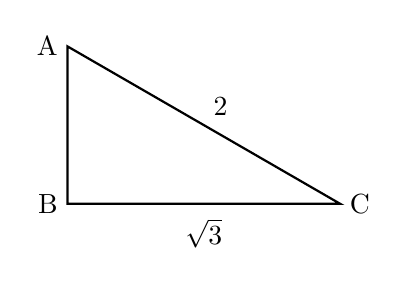
\begin{tikzpicture}[scale=2]
    % Define coordinates
    % Height = 1, Base = sqrt(3) approx 1.732, Hypotenuse = 2
    \coordinate (B) at (0,0);
    \coordinate (C) at ({sqrt(3)},0);
    \coordinate (A) at (0,1);

    % Draw the triangle
    \draw[thick] (A) -- (B) -- (C) -- cycle;

    % Vertex Labels (positioned slightly off the corners)
    \node[left] at (A) {A};
    \node[left] at (B) {B};
    \node[right] at (C) {C};

    % Hypotenuse Label
    \path (A) -- (C) node[midway, above right] {2};
    
    % Base Label
    % explicit 'below' distance ensures it doesn't touch the line
    \path (B) -- (C) node[midway, below=2pt] {$\sqrt{3}$};

\end{tikzpicture}

\end{document}